% This example An LaTeX document showing how to use the l3proj class to
% write your report. Use pdflatex and bibtex to process the file, creating 
% a PDF file as output (there is no need to use dvips when using pdflatex).

% Modified 

%\documentclass{article}
%\begin{document}
%\title{User Interface Evaluation}
%\author{Tony Lau}
%\maketitle
%==============================================================================
\section{User Interface Evaluation Methods}
\label{evalmethods}

The simulator will be evaluated through a series of user tests with different participants. The goals of the user interface evaluation are to assess the effect of the interface on the user and to identify specific problems which should be rectified. The simulator will be first tested with the fire warden of The Tall Ship who is the primary user of the system. Secondly, feedback on usability of the system will be gathered from usability testing with the subjects being students at the University of Glasgow.

Two evaluation methods, namely Heuristic Evaluation and Usability Experiments, will be used to determine whether the requirements specified in the Requirements chapter have been met and also to determine the overall usability of the system.

\subsection{Heuristic Evaluation}
Heuristic evaluation is a usability inspection method pioneered by Jakob Nielsen and Rolf Molich which helps to identify problems with a user interface by judging the interface's compliance to recognized usability principles -- heuristics\cite{heuristics}.

The heuristics made use of in this part of the evaluation are Nielsen's Heuristics, developed by Jakob Nielsen and Rolf Molich in 1990\cite{tenheuristics}. Nielsen refined the original set of heuristics in 1994\cite{tenheuristics}. Below is list of the heuristics and a description of each one:
\\
\textbf{1. Visibility of system status:}
The system should always keep users informed about what is going on, through appropriate feedback within reasonable time.
\\
\textbf{2. Match between system and the real world:}
The system should speak the user's language, with words, phrases and concepts familiar to the user, rather than system-oriented terms. Follow real-world conventions, making information appear in a natural and logical order.
\\
\textbf{3. User control and freedom:}
Users often choose system functions by mistake and will need a clearly marked "emergency exit" to leave the unwanted state without having to go through an extended dialogue. Support undo and redo.
\\
\textbf{4. Consistency and standards:}
Users should not have to wonder whether different words, situations, or actions mean the same thing. Follow platform conventions.
\\
\textbf{5. Error prevention:}
Even better than good error messages is a careful design which prevents a problem from occurring in the first place. Either eliminate error-prone conditions or check for them and present users with a confirmation option before they commit to the action.
\\
\textbf{6. Recognition rather than recall:}
Minimize the user's memory load by making objects, actions, and options visible. The user should not have to remember information from one part of the dialogue to another. Instructions for use of the system should be visible or easily retrievable whenever appropriate.
\\
\textbf{7. Flexibility and efficiency of use:}
Accelerators -- unseen by the novice user -- may often speed up the interaction for the expert user such that the system can cater to both inexperienced and experienced users. Allow users to tailor frequent actions.
\\
\textbf{8. Aesthetic and minimalist design:}
Dialogues should not contain information which is irrelevant or rarely needed. Every extra unit of information in a dialogue competes with the relevant units of information and diminishes their relative visibility.
\\
\textbf{9. Help users recognize, diagnose, and recover from errors:}
Error messages should be expressed in plain language (no codes), precisely indicate the problem, and constructively suggest a solution.
\\
\textbf{10. Help and documentation:}
Even though it is better if the system can be used without documentation, it may be necessary to provide help and documentation. Any such information should be easy to search, focused on the user's task, list concrete steps to be carried out, and not be too large.\\

The user interface of the simulator will be examined and evaluated using the descriptions of each of Nielsen's 10 Heuristics above. Heuristic Evaluation is a relatively quick and inexpensive way to evaluate a user interface. Deviation from recognized usability principles, identified from the evaluation, can provide great insight into how the user interface could be further refined to enhance the usability of the system.

\subsection{Usability Experiments}
Usability experiments can be used in addition to Heuristic Evaluation to gain further feedback on the system. These are particularly useful because they allow the experimenter to gain insight to the reactions of the users of the system first-hand.

Two different sets of users will be used for evaluation: the Tall Ship's fire warden and a group of students. The fire warden will be able to tell us whether the system meets the requirements and also on how usable the system is. Since it is unlikely that the students work in the domain of fire safety, the set of students will be primarily used to test the ease in which the system can be used. Any suggestions of improvements to the system by either group will also be recorded.

\subsubsection{Experimental Design}
The experiment must be designed carefully in order to provide results that are both reliable and generalisable. Two types of experimental design can be used: within-subjects design and between-subjects design.

In a between-subjects (or randomized) design, each participant is given a different condition, of which there are at least two. A control condition, where the independent variables are not changed, is needed to ensure the measured differences in the other conditions are true. Since each subject only performs under one condition, the likelihood of any learning effect from performing two similar conditions one after the other is mitigated. However, a between-subjects design requires a large number of participants if one is going to extract meaningful information.

In a within-subjects design, each subject is given the same conditions to perform. The effect of learning is more prominent in this method, which is a disadvantage but it has an advantage compared to between-subjects design because less subjects and time are required.

Considering the advantages and disadvantages of both methods, a within-subjects design will be adopted for the user interface evaluation of the evacuation simulator. Since limited resources are available in terms of time and users, the less costly within-subjects design is more appropriate. Learning effects can be lessened by changing the order in which the conditions are carried out by the participants. This allows a comparison of participants who carried out a condition first and participants who carried out the condition after another one, and therefore subject to learning. The results from the within-subjects evaluation will be analysed to determine whether effects of learning have adversely affected the results of the evaluation.

For both sets of users, they will carry out a set of fixed tasks and the time taken to perform these tasks as well as any mistakes they make will be recorded. This data will be used to form the evaluation results and will allow the identification of flaws in the usability of the system and areas for improvement.

\subsubsection{Think-aloud Protocol}
In addition to the usability experiment discussed above, the think-aloud protocol will also be used to gather information from users of the system. This method was introduced in the usability field by Clayton Lewis and is discussed in Task-Centered User Interface Design: A Practical Introduction by C. Lewis and J. Rieman\cite{uidesign}. Think-aloud protocols involve participants thinking aloud as they perform a set of pre-specified tasks. The idea is to have the users of the system saying out loud exactly what they are doing and how they are feeling. This allows the experimenter to gain a first-hand sight of a user using the product and provides insightful knowledge into how the end user would go about performing tasks.

The information gathered from the experiment will be analysed and the difficulties the user had will be discussed and rectified by changing the user interface. Any major changes to the user interface will have to be evaluated again to ensure the changes actually improve the usability of the system as a whole. 

\subsection{NASA TLX: Task Load Index}
%\begin{itemize}
%\item NASA TLX was used after the Think Aloud evaluation to measure the workload of the participants relating to the tasks that they had just performed. Talk about what it is and how it measures workload.
%\item Include pictures of the rating scale and the description of the rating scale from the instruction manual.
%\item Discuss the pairwise comparison and whether to use Raw TLX (RTLX). Cite 20 years later paper.
%\end{itemize}

NASA Task Load Index (TLX) will be used to measure the workload of the participants relating to the tasks that they are asked to perform. It is a subjective workload assessment tool which is used to derive an overall workload score based on a weighted average of the six subscales, namely Mental Demands, Physical Demands, Temporal Demands, Own Performance, Effort and Frustration\cite{tlx}.

\begin{figure}[H]
	\centering
	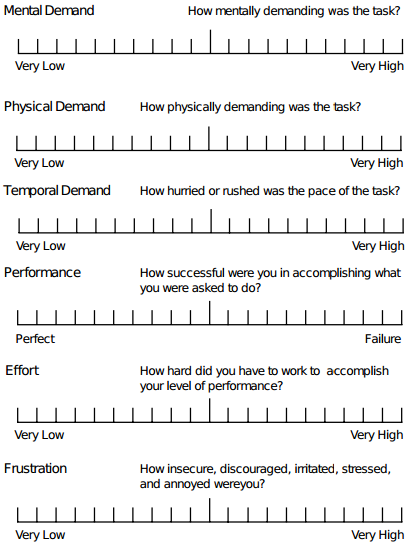
\includegraphics[scale=0.4]{../images/ratingscale.png}
	\caption{NASA TLX Rating Scales}
\end{figure}

After the participants have given a rating on each of the six subscales, they are asked to carry out a pairwise comparison between the subscales to identify their relative importance, in the eyes of the user.

This particular experiment involves asking the user to carry out pairwise comparisons, however, some research has suggested that the exclusion of the pairwise comparisons between subscales can increase experimental validity\cite{tlxinvariance}.

%==============================================================================================
\section{User Interface Evaluation Results}
\label{results}

The results from the user interface evaluation using heuristic evaluation, think-aloud and NASA Task Load Index (TLX) are discussed below. The recommendations in this section were used to enhance the Graphical User Interface which is discussed in section \ref{guidesign}.

\subsection{Heuristic Evaluation}
\subsubsection{Visibility of system status}
The system gives users little information about what is going on. For example, on pressing the populate or route buttons, no information is displayed on the screen informing the user that something is happening in the background. As a result, the user could be left wondering whether the button was correctly clicked.

Inclusion of messages on the screen stating what is happening at a particular moment in time would help the users to identify the status of the system. For example, inclusion of a message saying that the system is loading instead of a black screen will inform the user that something is indeed happening. Messages when the user clicks a button confirming that the action is happening and a message that displays on the screen when the evacuation simulation has finished will also increase the user’s awareness of the system status which in turn makes the system more user friendly.

\subsubsection{Match between system and real world}
The arrow keys (up, down, left and right) for camera movement are positioned in a logical order which would be familiar to the majority of users. This allows an easy mapping from real world natural conventions to the system which makes the system easier to use. Non-natural placement of these buttons on the screen would cause confusion in users and lead to frustration.

The system does use the term `navmesh' in the checkbox labelled `show navmesh'. The user is likely to be unfamiliar with this technical term and would thus have to consult the documentation to learn properly what it does. The system should use words and phrases familiar to the user so it would seem appropriate to replace the word `navmesh' with something along the lines of `ship outline' or `wireframe'.

\subsubsection{User control and freedom}
The user has the ability to control the camera manually using the on-screen buttons. The allows the user to view the ship in any way they want. There is also functionality to increase or decrease the speed of the camera and also to select preset camera locations from a drop-down menu which increases the control and freedom the user has. The number of preset camera locations is currently two. This should be expanded to give the user more options.

The user can change the population size from the main screen and a more advanced settings menu allows the user to create categories of people according to various factors. This gives advanced users more freedom in the interactions they make with the system.

\subsubsection{Consistency and standards}
In general, the buttons are labelled well and the user does have to wonder what they do. However, some problems exist in the camera settings part of the main screen. There are two up arrows and two down arrows and their functionality is not made entirely clear to the user. One of the up arrows is to pan up and the other up arrow is to rotate upwards. This should be made clear to the user by either increasing the size of the button and including a meaningful button name, or include the information as text above the buttons on the camera controls panel itself.

\subsubsection{Error prevention}
Some steps have been taken to prevent the users from executing an action which would lead to an error in the system. The evacuate button is grayed out and is only allowed to be clicked by the user when the ship has been successfully populated. By stopping the user from performing this action until it is appropriate, allows the prevention of an illegal system state -- namely evacuating an empty ship.

Error prevention related to the other buttons was overlooked and should be corrected. Other buttons on the main panel of the user interface should also be grayed out when it would not be appropriate to click.

Where there exist fields which can be altered by the user (for example, the population size field) a maximum and minimum value has been defined to prevent the user from entering too high or too low a number. This eliminates the possibility that the system will enter a state which it cannot handle as a result of user input which protects the system from mistakes made by the user.

\subsubsection{Recognition rather than recall}
The main buttons on the user interface are made to be as self explanatory as possible, however one shortfall is the design of the camera location panel. As discussed in the consistency heuristic, it should be made more clear what these buttons actually do. This would remove the need of the user to consult documentation for help and would thus reduce the extent of recall from one dialog to the next.

\subsubsection{Flexibility and efficiency of use}
The system has the ability to cater for more experienced user as mentioned in the user control and freedom heuristic. There exists the ability for the more experienced user to change a variety of properties of the camera such as speed and location. There is also the ability to use the keyboard to navigate around the ship which would allow more experienced users to increase their speed of interaction with the system.

There is, however, no method of allowing the user to tailor frequent actions through the use of accelerators or custom keyboard shortcuts, for example. The addition of such features would increase development time and since the experienced users group is a minority, it would not be in the best interest to develop this feature at this time.

\subsubsection{Aesthetic and minimalist design}
The system has a main screen which includes the most often used actions, and a settings screen which includes extra functionality. This separation allows a less cluttered minimalist view in the main screen which is easier to comprehend for the user. The system had been designed to display elements positioned in a natural way, allowing the user to focus on using the system and not needing to familiarise themselves with the interface for too long.   

\subsubsection{Help users recognize, diagnose and recover from errors}
As mentioned in the prevention of errors heuristic above, some steps have been taken to prevent the user from making errors. However, since not all sections of the interface are removed from use when they are not supposed to be used, it is possible for a user to crash the system by pressing the buttons repeatedly. There are no friendly error messages to tell the user that something has went wrong -- they are presented with a black screen. This leaves the user wondering whether the system is busy in the background carrying out some task, or has crashed.

To resolve this problem, better messages should be displayed on the screen to the user to increase visibility of system status. This would eliminate any confusion from the user when using the system. A reset button should also be implemented as a last resort for the user to click if the system crashes for an undocumented reason. This will ensure robustness in the system and increase the user-friendliness as a whole.

\subsubsection{Help and documentation}
No help or documentation is provided to the user. While the majority of the system is, on the whole, quite intuitive to use, some parts such as the camera controls panel and the advanced settings dialog box would benefit from documentation.

Brief documentation on the basic parts of the interface and what each button does as well as more detailed documentation on the more complex parts of the system should be created to assist the user in using the system and making decisions.

\subsection{Think Aloud}
The Think Aloud evaluation of the user interface was carried out with eight participants. The participants were asked to complete the six tasks listed below and were encouraged to ‘think aloud’ during the evaluation. The participants were observed and notes were taken to allow a discussion of improvements which could be made to the user interface after the evaluation.
\\
\\
\textbf{Tasks}
\begin{enumerate}
\item Set the population size to 50. Populate the ship.
\item Hide the ship frame from view, then show it again.
\item Generate the exit routes for the population.
\item Change the camera angle so you have a bird's eye view of the ship.
\item Evacuate the ship. While the evacuation is taking place, change the camera view to face the exits of the ship.
\item Read out loud the time the simulation took and the number of people evacuated.
\end{enumerate}
A summary of the findings of the Think Aloud evaluation is discussed below. Detailed notes on a per-participant level are included in Appendix C.

\begin{itemize}
\item The visibility of system status was a clear shortfall as indicated by the participants. Particularly in tasks 1, 3 and 5 where buttons which required the user to wait after being pressed, the participant was left guessing whether anything was happening with the system or whether they had done something wrong.
\item The meaning of the camera location buttons was also not as clear as they should have been. Participants had to investigate what the buttons did and clear labelling would have solved this issue.
\item The participants had no difficulty identifying key information such as number of people evacuated and the time taken for the evacuation which confirms that the information is well visible and the labelling is unambiguous.
\item Identification of the completion of the evacuation was most often done by looking at whether anything more was happening in the graphical representation rather than looking at the `remaining people' metric at the right hand side of the interface. It was noted that a pop-up message when the simulation is complete would make this more clear to the user.
\item The terminology used in the user interface must be standardised to remove jargon words such as ‘navmesh’ which would be unclear to the user. Task 2 highlighted that while some users guessed that ‘ship frame’ was equivalent to the ‘navmesh’ in this particular situation, 5 of the 8 participants were confused by the technical language. 
\end{itemize}

\subsection{NASA TLX: Task Load Index}
%\begin{itemize}
%\item Insert graph.
%\item Discuss that there is a low workload in using the system.
%\end{itemize}

\begin{figure}[H]
	\centering
	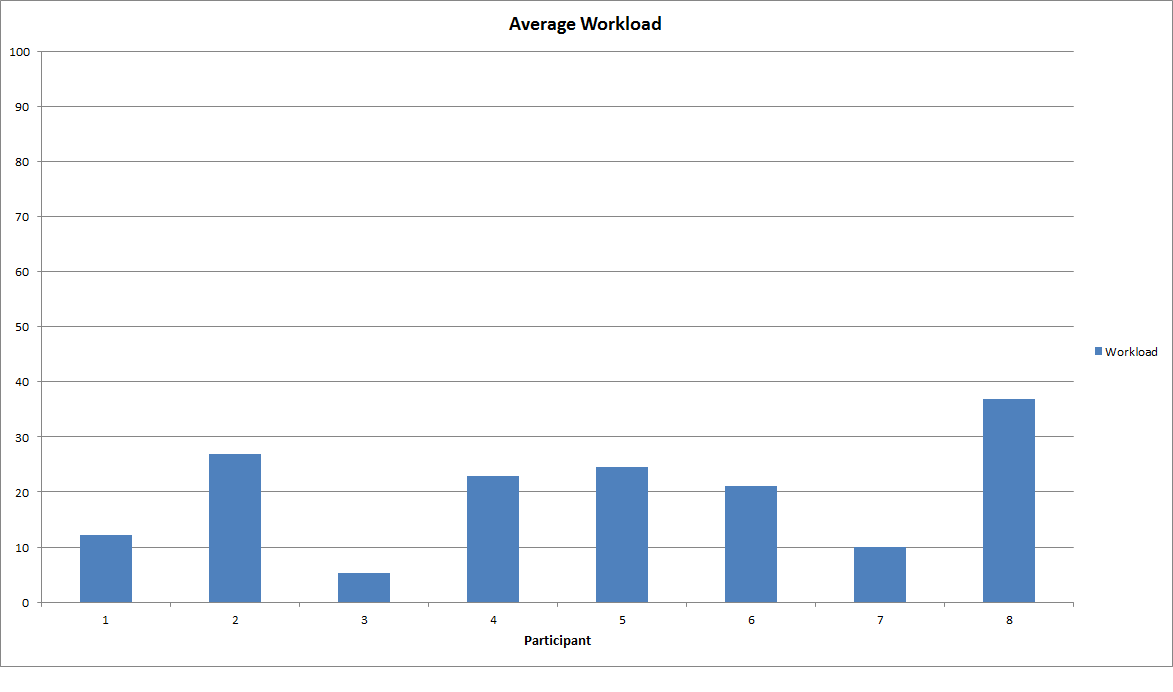
\includegraphics[scale=0.25]{../images/tlxresults.png}
	\caption{Average workload across participants}
\end{figure}

The above image shows the average workload of the eight participants in the experiment, which is calculated based on the ratings and pairwise comparisons given by the participant. It can be seen that the overall workload of each participant is reasonably low and so it can be said that using the system is not demanding. 

%==============================================================================================


%==============================================================================
%\end{document}
